\documentclass[12pt]{article}

% This first part of the file is called the PREAMBLE. It includes
% customizations and command definitions. The preamble is everything
% between \documentclass and \begin{document}.

\usepackage[margin=1in]{geometry}  % set the margins to 1in on all sides
\usepackage{graphicx}              % to include figures
\usepackage{subfig}
\usepackage{epstopdf}
\usepackage{amsmath}               % great math stuff
\usepackage{amsfonts}              % for blackboard bold, etc
\usepackage{amsthm}                % better theorem environments




\begin{document}

\begin{center}
{\bf \Large Visual Saliency: A Project Proposal}  \\
\vspace{.1in}
{\em Sijie Ling, Shupei Zhang, Mehdi Akbarian Rastaghi}
\end{center}
%\setlength\parindent{0pt}
\section{Introduction}

Visual saliency is the extent of attraction of objects to our visual system. 
The human visual system can focus on the most salient stimuli and pay less attention to the rest. 
For example, a running dog in a still background will attract more of our attention. 
A reason for developing such a feature is that the amount of data we receive through our eyes exceeds our ability to process data. 
Although human brain capabilities evolved through time, it is a big challenge for our brain to process this tremendous amount of data efficiently. 
Hence, visual saliency can help us to identify the most imminent threat, danger, or events needing our attention in general. 
Technically, it reduces the load on our visual system. 

The study of visual saliency can help us to have a deeper understanding of the human visual system. 
Researching in this area can lead to many applications, such as image/video segmentation, image/video compression, foreground annotation, perceptual quality assessment, etc \cite{congReviewVisualSaliency2019}.  
To shed more light, let's start with a case. 

Most of the current video coding methods are using block-based compression. 
As an example, spatial and temporal redundancy is reduced through intra-frame coding and inter-frame coding, respectively\cite{sullivanOverviewHighEfficiency2012}. 
While these methods play a vital role in the comparison area, video encoders can further increase the compression ratio by incorporating visual saliency models. 
This can be achieved by decreasing the quality of regions of low interest, like the background. 
Because it is hard for us to notice the changes in those regions, the perceptual visual quality will likely remain the same.

Another advancement of visual saliency is in the game industries. 
Visual saliency study might help game developers in optimizing the performance of their games. 
Due to the difference in attraction of different regions, not all areas need to be rendered in the highest quality, which leads to a better graphics performance. 
Therefore, considering all contribute of visual saliency techniques motivates us to do some research in this area. 

In this project, we will explore how to use attention mechanisms in computer vision, like \cite{zhangSelfAttentionGenerativeAdversarial2019a},
to help capture global dependencies, and thus improve the saliency prediction performance. 
The model will be an end-to-end model, where the input is a color image and the output is a saliency map.
The saliency map is the same size as the input image, with scores from 0 to 1 assigned to 
every pixel, indicating the extent of attraction of the corresponding pixel in the input image.
Higher values correspond to higher visual saliency levels.
One example of the original image and its corresponding saliency map is shown in Fig. \ref{img:data_example}.
\begin{figure}[!h]
    \centering
    \subfloat[][Original]{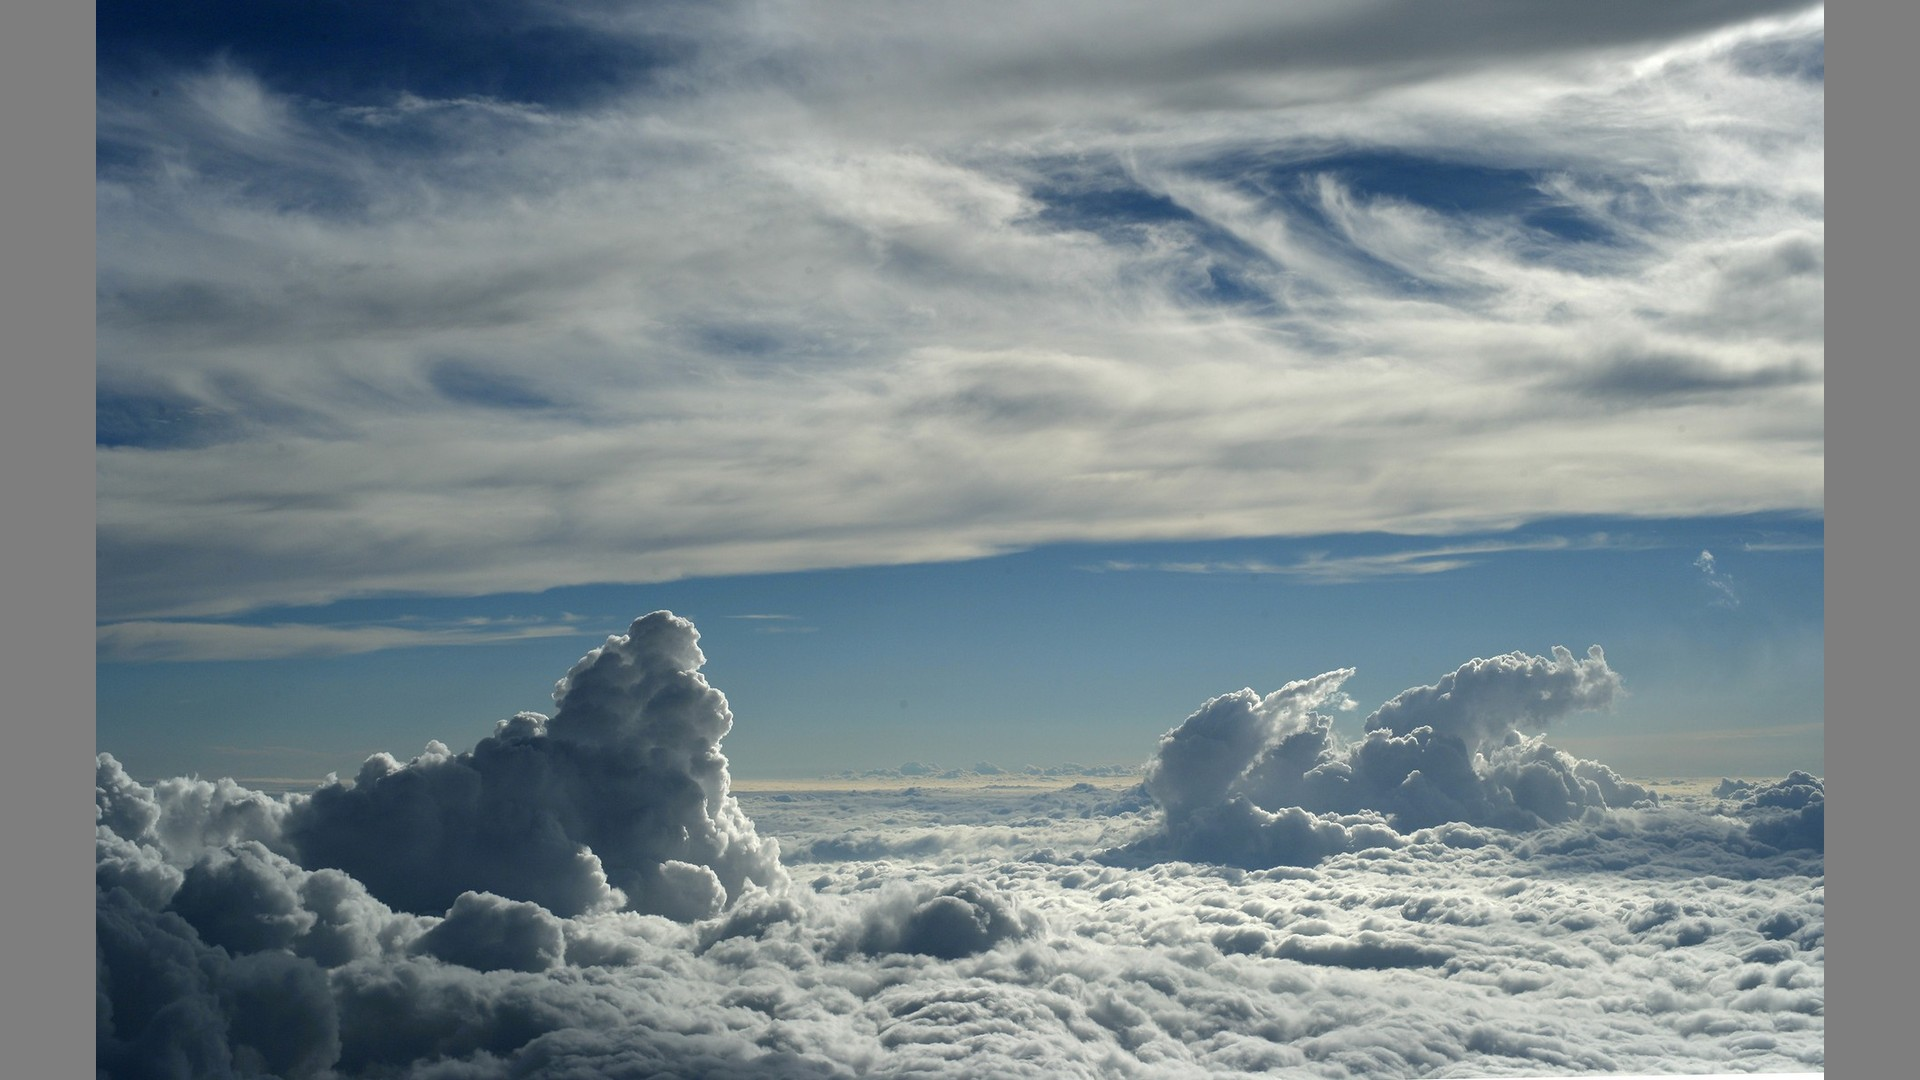
\includegraphics[width=3in]{imgs/example1_original.jpg}}
    \hspace{5mm}
    \subfloat[][Saliency map]{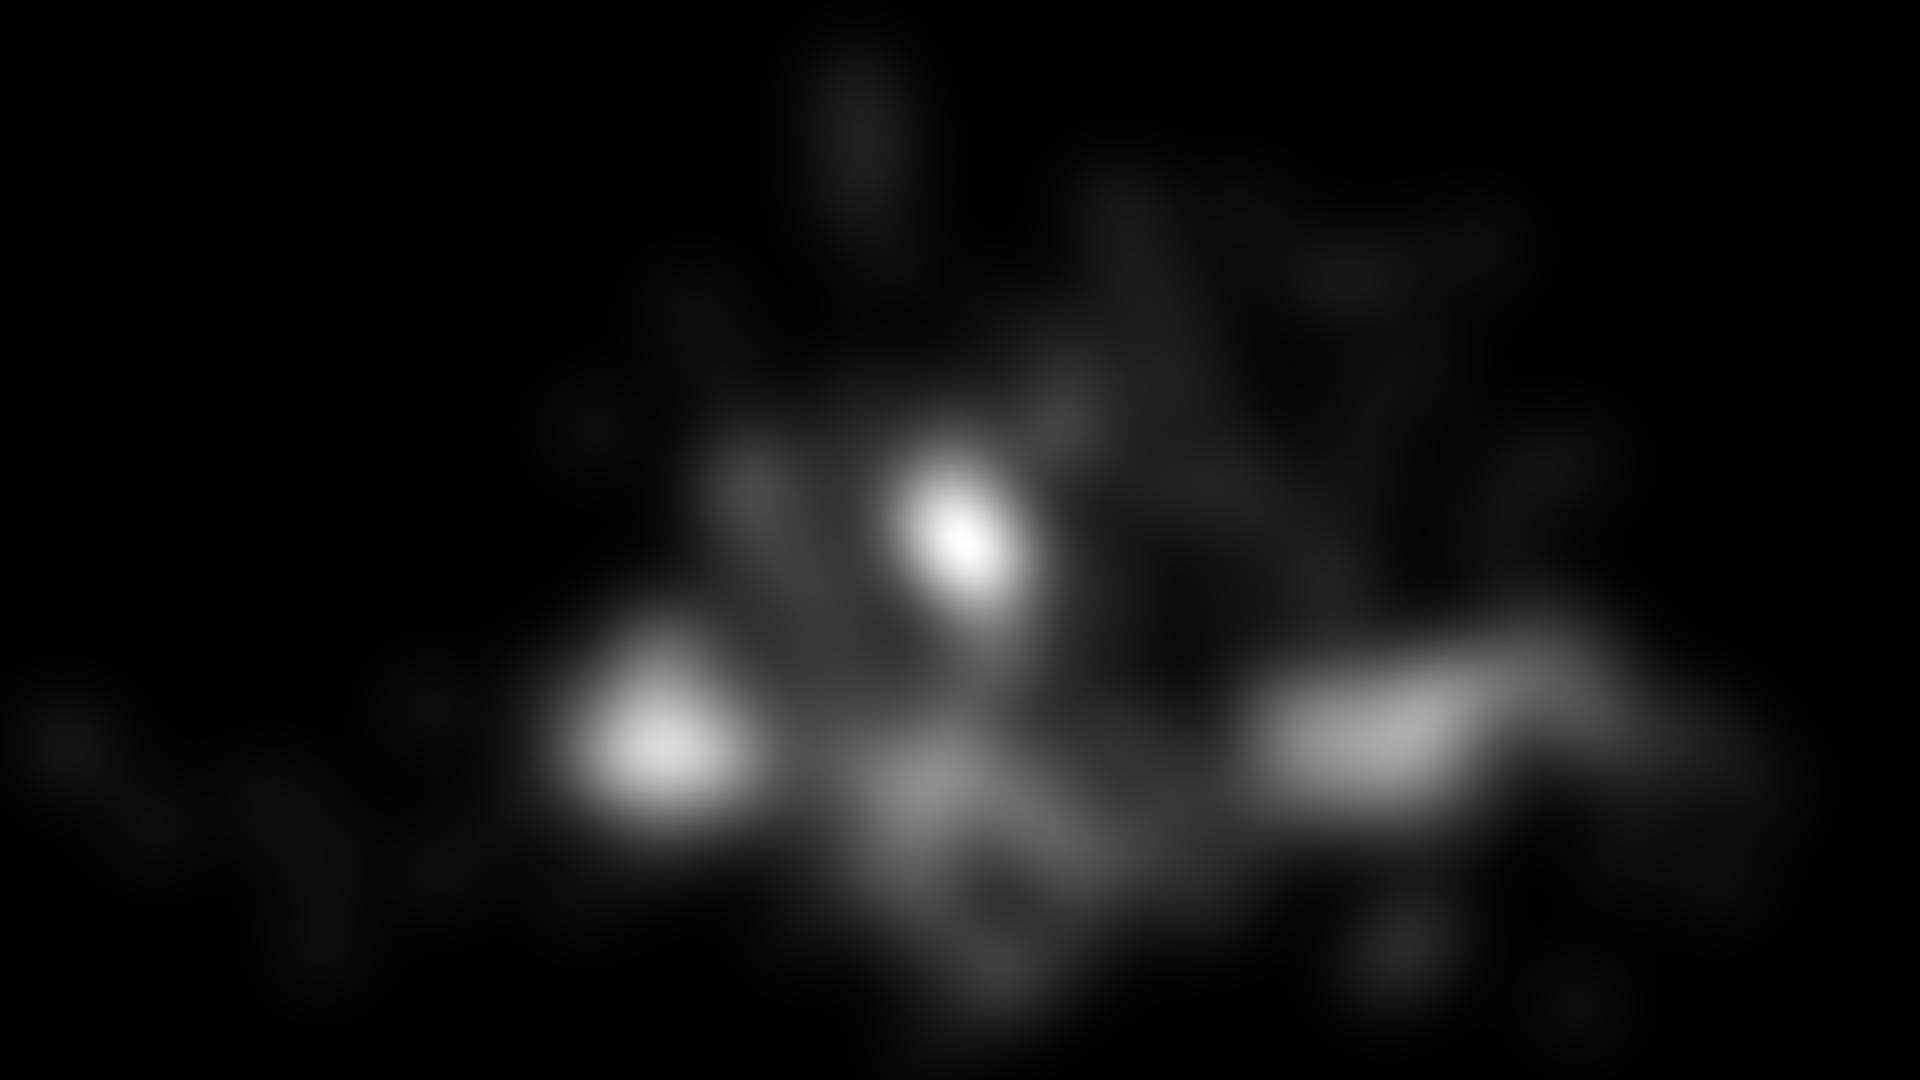
\includegraphics[width=3in]{imgs/example1_saliency.jpg}}
    \caption{Data example}
    \label{img:data_example}
\end{figure}


\section{Related Work}

Visual saliency detection methods can be categorized into two two classes: bottom-up models and top-down models \cite{congReviewVisualSaliency2019}.
Before deep learning was widely applied in this field, most of the early methods are bottom-up models.
Those early methods usually involve biological and psychological research about visual attention mechanism. And those two approaches match the common beliefs about biological process of human vision.
In general, those models try to establish links between visual saliency and low-level image features, such as color, contrast, brightness etc. The Itti. model\cite{ittiModelSaliencybasedVisual1998}
is one of the earliest model of this kind, which predicts visual saliency from linear combination of features calculated from color, intensity and orientation.
Some other techniques are also used to achieve better results, such as frequency domain analysis, sparse representation, cellular automata etc. \cite{congReviewVisualSaliency2019}

Top-down models, in the other hand, try to find what factors have the most impact on visual saliency. Those models use visual saliency datasets, which contain images and their saliency annotations
, and analyze them in a data-driven fashion.
In recent years, deep learning is introduced into this area and has boosted the performance of saliency prediction a lot.
Vig et al. \cite{vigLargeScaleOptimizationHierarchical2014} proposed the first neural network for saliency prediction, combining convolutional neural network (CNN) and support vector machine (SVM). Later, researchers start to use transfer learning for saliency 
detection tasks. Very deep convolutional networks (VGG) is used in multiple models \cite{kruthiventiDeepFixFullyConvolutional2015, kummererDeepGazeIIReading2016, corniaPredictingHumanEye2018}, and some of them incorporate gaussian prior for performance improvement.
Generative adversarial networks also achieve good results in saliency prediction \cite{panSalGANVisualSaliency2018, cheHowGazeInfluenced2020}.

Transformer is a network based on attention mechanisms, ans is first applied in natural language processing (NLP) for its ability to model long range and multi-level information \cite{bahdanauNeuralMachineTranslation2016a, vaswaniAttentionAllYou2017a}.
They are later introduced for computer vision tasks and show strong potential in modeling non-local dependencies in images \cite{zhangSelfAttentionGenerativeAdversarial2019a}.
But this technique has not been applied in visual saliency tasks so far.

Our trial of applying attention mechanism to CNNs to improve the performence also has supporting evidence from the aspect of cognitive psychology. There are two contradictory models that try to explain human attention mechanism \cite{gazzaniga2006cognitive}. 
In the “Early Selection Model”, complete analysis is not necessary for an unimportant stimulus before it is excluded from our focus area, while in the “Late Selection Model”, all the stimuli are equally processed until they reach at least the semantic level. 
Both models have evidence and the key to solving the divergence is to find the threshold between them. From this view, since CNN usually have small receptive fields in the first few layers, the information is highly abstract for high level analysis, so traditional models can be regarded as similar to the late selection. 
The computer vision attention mechanism focuses more on global information, and we guess that its low level of preprocessing can ease the burden of CNN and guide it to a better result.

\section{Data}
\subsection{Datasets}

The datasets that are commonly used for image saliency prediction tasks are MIT1003 \cite{judd2012benchmark}, CAT2000 \cite{borji2015cat2000} and SALICON \cite{jiang2015salicon}.
In all three datasets, the original data are normal pictures. Grey margins are attached to some of the pictures to make them the same size. 
The labels, or the training targets are heatmaps that highlight some regions that are of interest to human.
Generally, those datasets are created using eye-tracking devices or mouse tracking software. The trajectories of eye/mouse movement while
observing the test images are recorded, and fixation maps can be created
by placing the trajectories as white pixels on black backgrounds. Saliency maps are generated by
applying a gaussian filter to the fixation maps and then normailize the results to range $[0, 1]$.
Fig. \ref{img:data_example_2} shows one example from SALICON dataset, of the original image, its corresponding 
fixation map, and the saliency map created by applying gaussian blur to the fixation map with $\sigma=19$.
\begin{figure}[!h]
    \centering
    \subfloat[][Original]{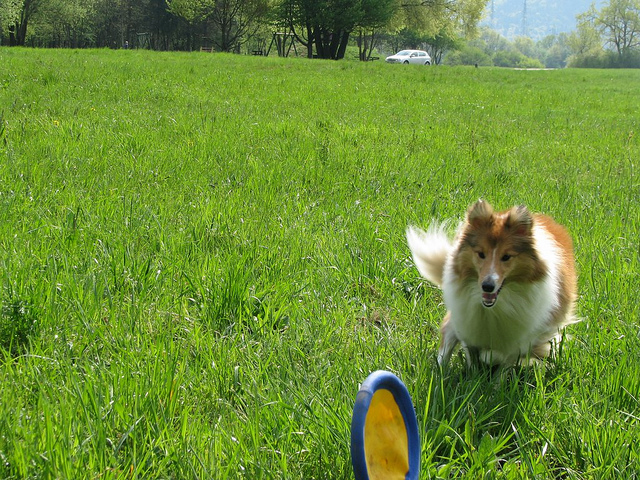
\includegraphics[width=2.5in]{imgs/example2_original.jpg}}
    \hspace{1mm}
    \subfloat[][Fixation map]{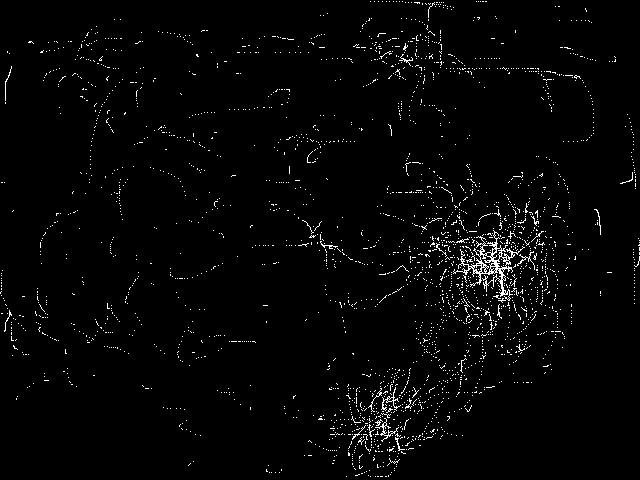
\includegraphics[width=2.5in]{imgs/example2_fixation.png}}
    \hspace{1mm}
    \subfloat[][Saliency map]{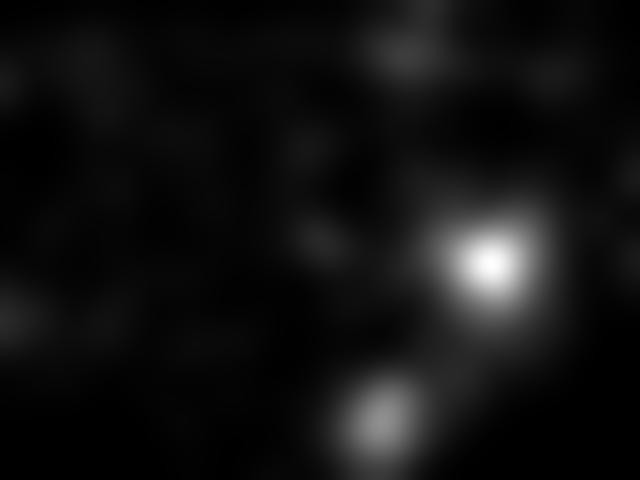
\includegraphics[width=2.5in]{imgs/example2_saliency.jpg}}
    \caption{Data example}
    \label{img:data_example_2}
\end{figure}

The MIT1003 dataset contains 1003 images, including 779 landscape images and 228 portrait images.
The data is collected from 15 observers using a 240Hz eye-tracker during a 3 second period of 
free viewing. The original images, eye-tracking data and fixation maps are available in this dataset.

The CAT2000 contains 4000 images from 20 different categories. In those images, 2000 are for training and the other 2000
are for testing. There are 24 test subjects for each image and a total of 120 test subjects. The free 
viewing duration is 5 seconds. Fixation data from only 18 out of 24 test subjects are available in training
set, and the test set is released with only the original images.

The SALICON dataset is created using images from Microsoft Common Objects in Context (MS COCO) dataset\cite{linMicrosoftCOCOCommon2015}.
Instead of using a eye-tracker, mouse trajectories from different viewers are used in this dataset 
to calculate probability distribution of visual attention. A total of 20000 images from 80 categories, including
10000 in training set, 5000 in validation set, and 5000 in test set.
In training set, the original images, fixation maps, and saliency maps are all available, while 
the test set is released without fixation maps and saliency maps.


We plan to combine the training and validation set of SALICON, 
and split it into 10 folds(7 for training, 2 for validation, and 1 for testing). 
Our training data is
\begin{itemize}
    \item 7 folds from SALICON
    \item training set of CAT2000.
\end{itemize}
Our validation data for tuning the hyper-parameters is the other 2 folds from SALICON, 
and our testing data consists the remaining 1 fold from SALICON together with MIT1003.


\subsection{Interpretability}

The visual saliency algorithm takes an input of the original figure, and outputs a saliency map of the same size. Each pixel contains a float number from 0 to 1. Bigger numbers show that these pixels or areas get more focus. Therefore, it is a regression task and the output can be visualized by plotting the saliency map.
However, we are still interested in what information in the picture is used by the algorithm to calculate the output. Some pixels, like sharp margins, may help locate the focused area, but may not be themselves focused.
Therefore, gradients methods \cite{sundararajan2017axiomatic} can be used to determine which pixels have the most contribution to determine the focused areas.

Moreover, we are doing analysis on existing CNN framework and use attention mechanism as a part of our framework. Since we previously have the assumption that convolution layers are good at processing local and abstract information while attention mechanism uses global information to help improve the performance, we should carefully analyze the contributions of these two components. In the network, attention mechanisms will act as special layers that are inserted into the neural network and assign different weights to their inputs.
The first method is to disable the attention layers and see whether the performance becomes significantly worse. If it does, we will know that the inserted layers help improve the performance.
The second method is to disturb the attention layers, namely by creating random heat maps with similar distributions to misguide the network. If the result gets worse, we will know that the output depends much on these layers.

\section{Analysis}
\subsection{Algorithm}

We can use VGG, ResNet, MobileNet etc. as the backbone of our model, since existing models seem to be fairly simple. Before the picture is directly sent into the framework, an attention framework will firstly assign weights to different parts of the picture.
Another alternative is we can incorporate attention mechanism \cite{zhangSelfAttentionGenerativeAdversarial2019a} into saliency detection model.

Some datasets might not have heatmap groundtruth available, and different dataset might use different gaussian standard variance to create the heatmap.
So we might need to generate heatmaps using a set of uniformed parameters from fixation data.
The training process will be similar to that in most computer vision tasks. Input data is feeded to the model,
and the output is compared with groundtruth to compute loss. Loss is then backpropagated to update model parameters.
Since real test set of these data sets are not public, we will divide the original data set into the train set, the validation set and the test set. We can use choose suitable hyper-parameters based on the results of the train set and the validation set.


\subsection{Performance Measurement}

There are several metrics that can be used to measure the performance. According to \cite{riche2013saliency}, these various metrics may reflect different properties of the algorithm.
\begin{itemize}
    \item Normalized scanpath saliency (NSS \cite{petersComponentsBottomupGaze2005})
    \item Correlation coefficient (CC)
    \item Area under receiver operating characteristic curve(AUC \cite{richeSaliencyHumanFixations2013})
    \item etc.
\end{itemize}

The NSS measures the mean saliency value at fixated locations of the normalized (zero mean, unit variance) saliency map. 
It can be calculated using Eq. \ref{EQ:NSS}. 
\begin{equation}
    \begin{aligned}
        NSS &= \frac{\sum^{N} T_{i}}{N}\\
        \text{where }T &= \frac{S - \bar{S}}{\sigma_{S}} \circ F
    \end{aligned}
    \label{EQ:NSS}
\end{equation}
In this equation, $S$ is the saliency map, $\bar{S}$ is the mean of $S$, $\sigma_{S}$ is 
the standard deviation of $S$, $F$ is the fixation map with only $0$ and $1$ as pixel values in it,
$T_{i}$ is the pixel value in $T$ at location $i$, and $N$ is the total number of non-zero pixels in $F$.

The CC is the linear correlation coefficient between a model saliency map and an empirical saliency map 
gained from convolving the fixation locations with a Gaussian kernel. It can be calculated using EQ. \ref{EQ:CC}. 
\begin{equation}
    \begin{aligned}
        CC = \frac{\sum_{i=1}^{n}(x_{i}-\bar{x})(y_{i}-\bar{y})}
        {\sqrt{\sum_{i=1}^{n}(x_{i}-\bar{x})^{2}}\sqrt{\sum_{i=1}^{n}(y_{i}-\bar{y})^{2}}}
    \end{aligned}
    \label{EQ:CC}
\end{equation}


In AUC metric,
the saliency map is treated as a binary classifier to separate positive from negative samples at various thresholds. 
The true positive (TP) rate is the proportion of saliency map values above threshold at fixation locations. 
The false positive (FP) rate is the proportion of saliency map values above threshold at all pixels. 
We calculate the TP rate and FP rate using a series of thresholds between $[0, 1]$, and draw a
receiver operating characteristic (ROC) curve with FP rate as x-axis and TP rate as y-axis.
An example of this curve is shown in Fig. \ref{img:AUC} \cite{hanleyMeaningUseArea1982}.
The area under this curve is reported as AUC.
\begin{figure}[!h]
    \centering
    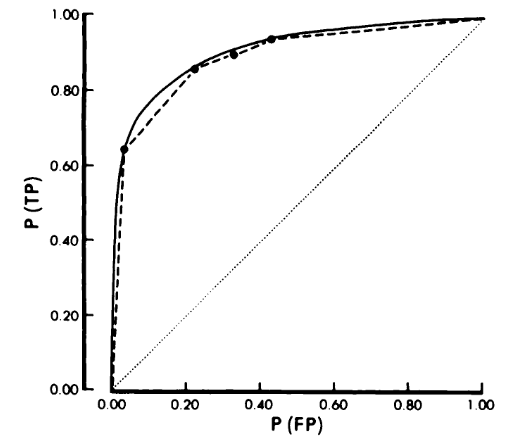
\includegraphics[width=2.5in]{imgs/AUC.png}
    \caption{ROC curve example}
    \label{img:AUC}
\end{figure}


The performance is reported on the testing fold of SALICON and also the whole MIT1003 dataset.
Reporting scores using different datasets can make the results more convincing,
because it can show that our model can generalize well.

\subsection{Further Verification}

For the trained network, we may first disable the attention mechanism and compare the several metrics of the output saliency map with the CNN networks without attention mechanisms.
This step will show the contributions of attention layers. If the metrics above have different levels of changes, we will infer about the properties of the attention layers according to the characteristic of these metrics.

The second step is to find out why attention mechanism may help improve the performance. 
During the test process, upon the output of attention mechanism, we can add noise or create random weights to misguide the CNN network to see whether the result is largely influenced.
This step can show whether the final output depends largely on attention mechanism.

If time permitting, we might also use the Integrated Gradients algorithm (IG) \cite{sundararajan2017axiomatic} to analyze what pixels in the picture contributes to the result. 
It might be interesting if we can find some pixels that are not highlighted but help the machine to focus. 
Besides, since the IG algorithm measures the gradient change from a totally dimmed picture to the original one, we can test the sensitivity of our algorithm.

\section{Work Plan}

Step1: Before the March 4 checkpoint, we are going to write the code of the CNN network and applies attention mechanism to it. 
If time permitting, we can try two or three attention mechanisms that are differently defined to see whether there are some differences. 

Step2: Before March 25, interpretability analysis will be done on the trained model. Details include cross validation to test both the final output and the influence of attention mechanism. 

Step3: Before we submit the final report, we are going to use some other tools to find some other aspects of our model. 
For example, whether there are some pixels that are not focused but help to achieve the final output and how our model will respond to dimmed pictures. 

\newpage

\bibliographystyle{unsrt}
\bibliography{proposal}


\end{document}
